\chapter{Implementation}

\section{Architecture}

The architecture of our system is illustrated in Figure~\ref{fig:architecture}. Our system consists of two applications: a main application that runs on the developer's machine and a helper application that runs on the real devices. Both the main application and the helper application are pure web applications and are provided by a server that is also responsible for forwarding communication between the main application and the side applications running on real devices.

Additionally, a local DNS server runs on the developer's machine. It is responsible for creating different subdomains for the emulated devices. The DNS server is required for properly testing and debugging on emulated devices, but if only real devices are used, it is not needed and can be disabled in the options of our system.

\begin{figure}[H]
  \centering
    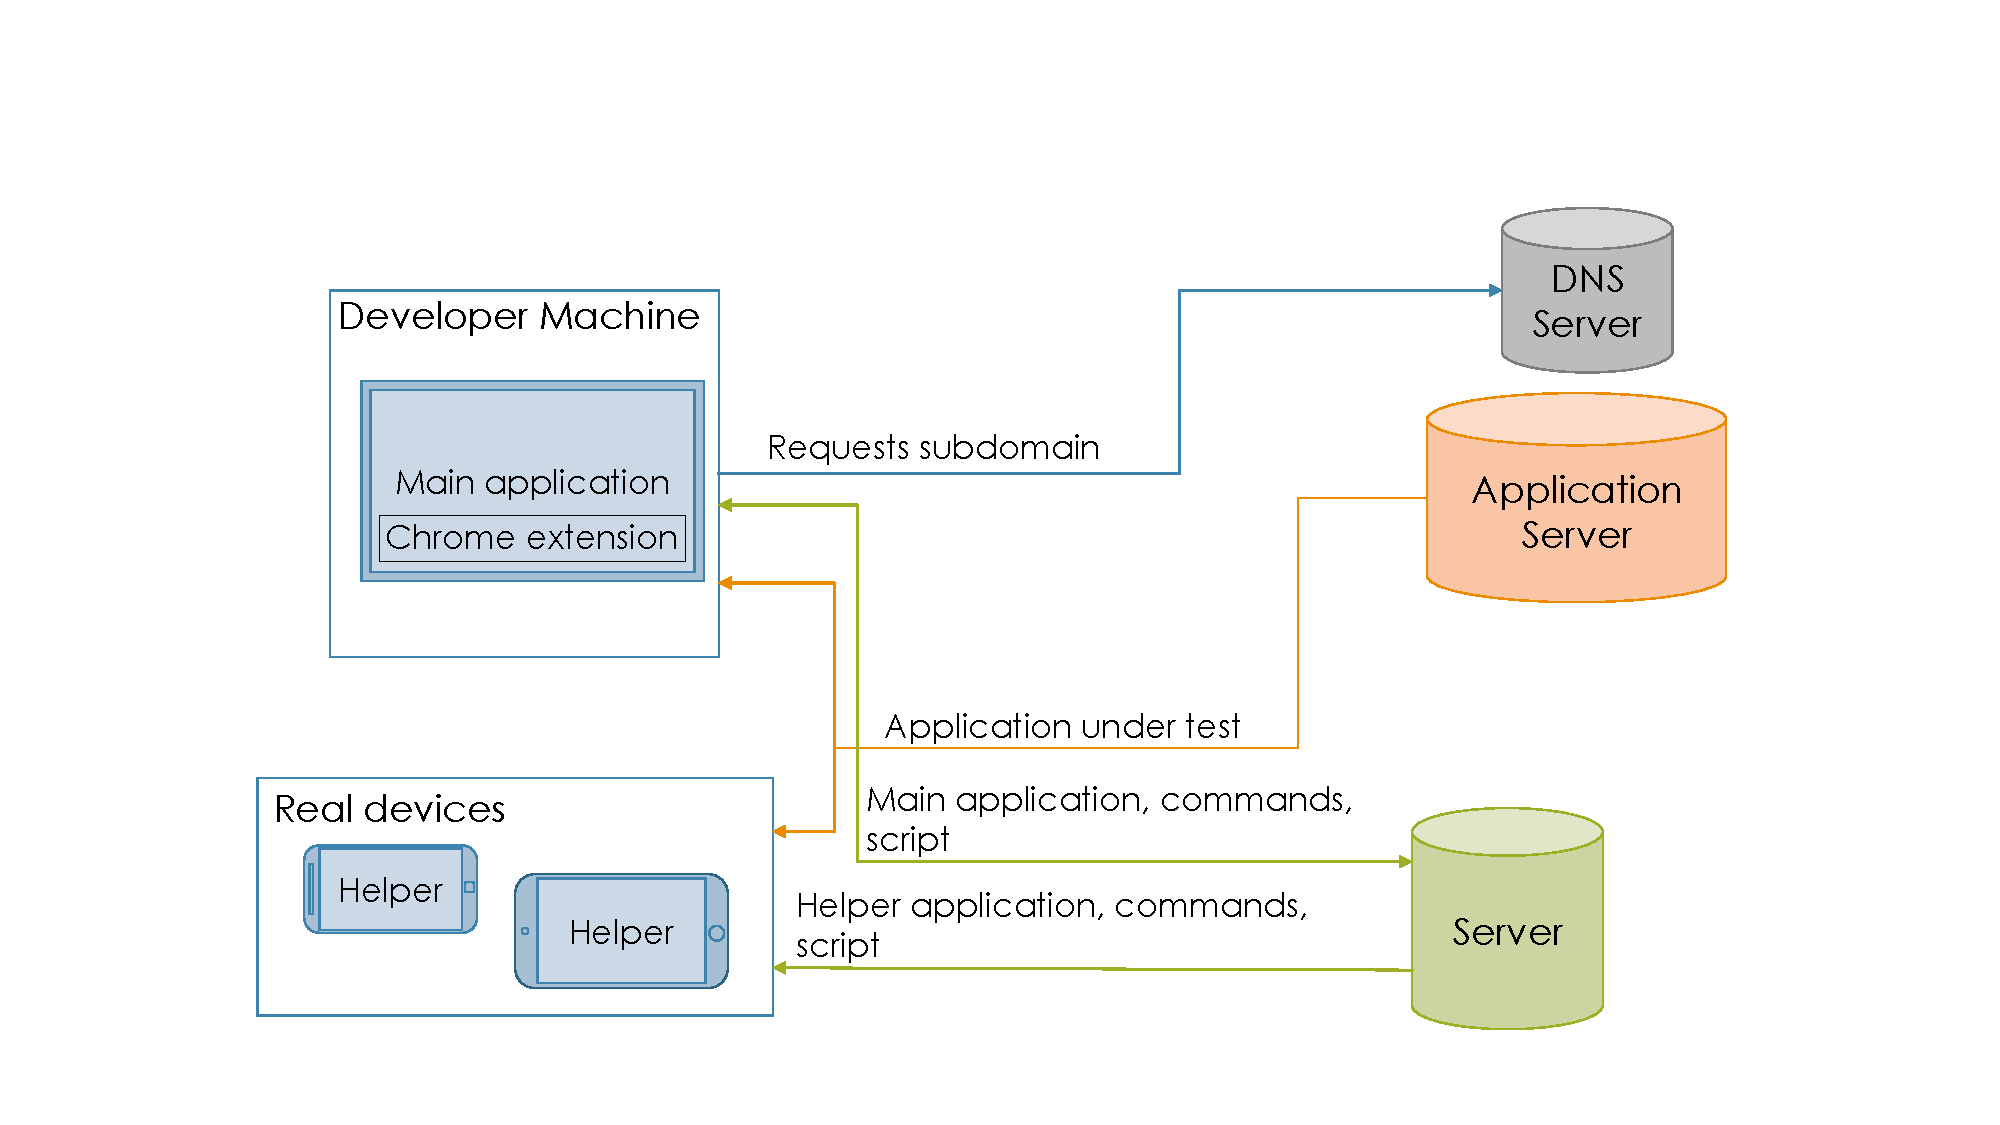
\includegraphics[width=1.0\textwidth]{images/architecture_2.pdf}
	\caption[Architecture of our system]{Architecture of our system}
	\label{fig:architecture}
\end{figure}

Furthermore, a Chrome extension runs in the browser of the developer's machine. This extension is needed for function debugging and inspection as well as HTML inspection. The Chrome extension communicates with the main application via the server.

Finally, some web server needs to provide the application under test. However, any web server can be used and our system does not place any restrictions. The only requirement is that the developer injects a small script that is hosted on our server at the top of each HTML page of the application. The script is responsible for performing many actions that would otherwise be difficult, such as executing JavaScript, recording events and adding CSS to the application under test.

\section{Choice of Technologies}

Since our set of tools includes desktop devices as well as mobile devices, it should be platform-independent. Thus, our tools are implemented using standard web technologies, i.e. HTML5, CSS3 and JavaScript. This allows our tools to be run in any modern web browser without requiring installation of any additional software. The fact that cross-device applications are also typically web-based makes web technologies even more suited for our tools. Our tools do not rely on any database, instead HTML5 Local Storage\footnote{\url{http://www.w3schools.com/html/html5_webstorage.asp}} is used for the data that we want to store. Our set of tools only need to store three things:
\begin{itemize}
	\item Custom devices for emulation that were added by the developer.
	\item Device configurations.
	\item Event sequences for replaying.
\end{itemize}
All those things only need to be accessed by the developer that created them. Thus, it makes sense to only store the data locally. Furthermore, the amount of data that needs to be stored is rather low and does not require much storage. 

\subsection{Server Side}

On the server side, our system uses Node.js\footnote{\url{https://nodejs.org/en/}}. Node.js is a JavaScript runtime that uses asynchronous I/O with an event-driven programming model. It is lightweight and scales well with a large number of connections. Furthermore, it has the advantage that both the client and server side are implemented using JavaScript. Thus, no data conversions are required. In our application, fast communication between the desktop PC and the connected real devices is required and Node.js fulfills those requirements. Node.js' package ecosystem, npm\footnote{\url{https://www.npmjs.com/}} provides a large number of modules which extend the capabilities of Node.js. We use the following modules in our system: 
\begin{itemize}
	\item Express\footnote{\url{http://expressjs.com/}}: Express is a minimal and flexible web application framework that provides a set of features for web and mobile applications. In our system, Express is responsible for serving the content to the clients.
	\item shortid\footnote{\url{https://github.com/dylang/shortid}}: shortid generates short URL-friendly unique IDs. shortid generates the device IDs for the emulated devices in our system. As each device gets a subdomain based on its ID, shortid is ideal for our purpose.
	\item Socket.IO\footnote{\url{http://socket.io/}}: Socket.IO enables real-time bidirectional event-based communication. If available, it uses HTML5 WebSockets, otherwise it uses fallback mechanism like AJAX long-polling. In our system, Socket.io is used for the communication between the server and clients.
\end{itemize}

Socket.io is better suited for our application than AJAX for multiple reasons: First, we need to be able to send push data to clients from the server for sending commands to devices and AJAX is intended to allow clients to pull data from the server. Also, data transfer with AJAX comes with a significant overhead because HTTP headers are transmitted with each piece of data. As we mentioned before, fast communication between the server and the devices is a requirement for our system and AJAX would not fulfill this requirement sufficiently. However, AJAX is used for communicating with the DNS server.

\subsubsection{DNS Server}

Our system requires a DNS server for registering the subdomains for the emulated devices. It should be easy to dynamically register new subdomains to the DNS server. Furthermore, the DNS server should forward any unknown domains to the standard DNS server. rainbow-dns\footnote{\url{https://github.com/asbjornenge/rainbow-dns}} fulfills both those requirements. It is a Node.js-based DNS server with an HTTP API that makes it trivial to register new domains from our application. When starting the server, the IP address of the standard DNS server can be passed as an argument, allowing rainbow-dns to forward unknown domains to the standard DNS server.

\subsection{Client Side}

The client side of our system is implemented using JavaScript with jQuery\footnote{\url{https://jquery.com/}}. jQuery allows easy selection and modification of HTML elements as well as easy event handling, features that are crucial to our system. As an additional helper, we use jQuery UI\footnote{\url{https://jqueryui.com/}}. jQuery UI is mainly used for the autocomplete functionality and for easy resizing of the individual components of our application. It is also used for resizing the emulated devices to change their resolution. The Twitter Bootstrap\footnote{\url{http://getbootstrap.com/}} framework is used to give our application a nice and uniform look-and-feel. It is also used for facilitating the implementation of things like modal boxes and tabs. 

Our system also uses QR codes for connecting real devices to the system. We use the jQuery-based QR Code library jQuery.qrcode\footnote{\url{https://larsjung.de/jquery-qrcode/}} for generating those QR codes. Using jQuery selectors, the content of an HTML element can be set to a QR code with the desired content and size.

HTML5 Drag and Drop\footnote{\url{http://www.w3schools.com/html/html5_draganddrop.asp}} is used for allowing accurate positioning of devices and timing of event sequences. HTML5 \lstinline|postMessage| is used for communication between the testing application in the \lstinline|iframe| and our application. Thus, no additional library for communication is needed inside the testing application.

The script that is injected into the application under test is implemented in pure JavaScript. Using libraries like jQuery inside this script could lead to conflicts with other libraries in the application under test or different versions of jQuery. Also, loading jQuery into the application creates some additional overhead and might not be what the developer of the application wants.

The Chrome DevTools extension is implemented using JavaScript. It uses the Command Line API\footnote{\url{https://developer.chrome.com/devtools/docs/console-api}} for accessing the functions needed to inspect HTML, debug functions, and more. The extension also uses Socket.IO for  communicating with the server. 

\section{Overview of Features}

In Figure~\ref{fig:complete}, the complete interface of our system except for record and replay can be seen.

\begin{figure}[H]
  \centering
    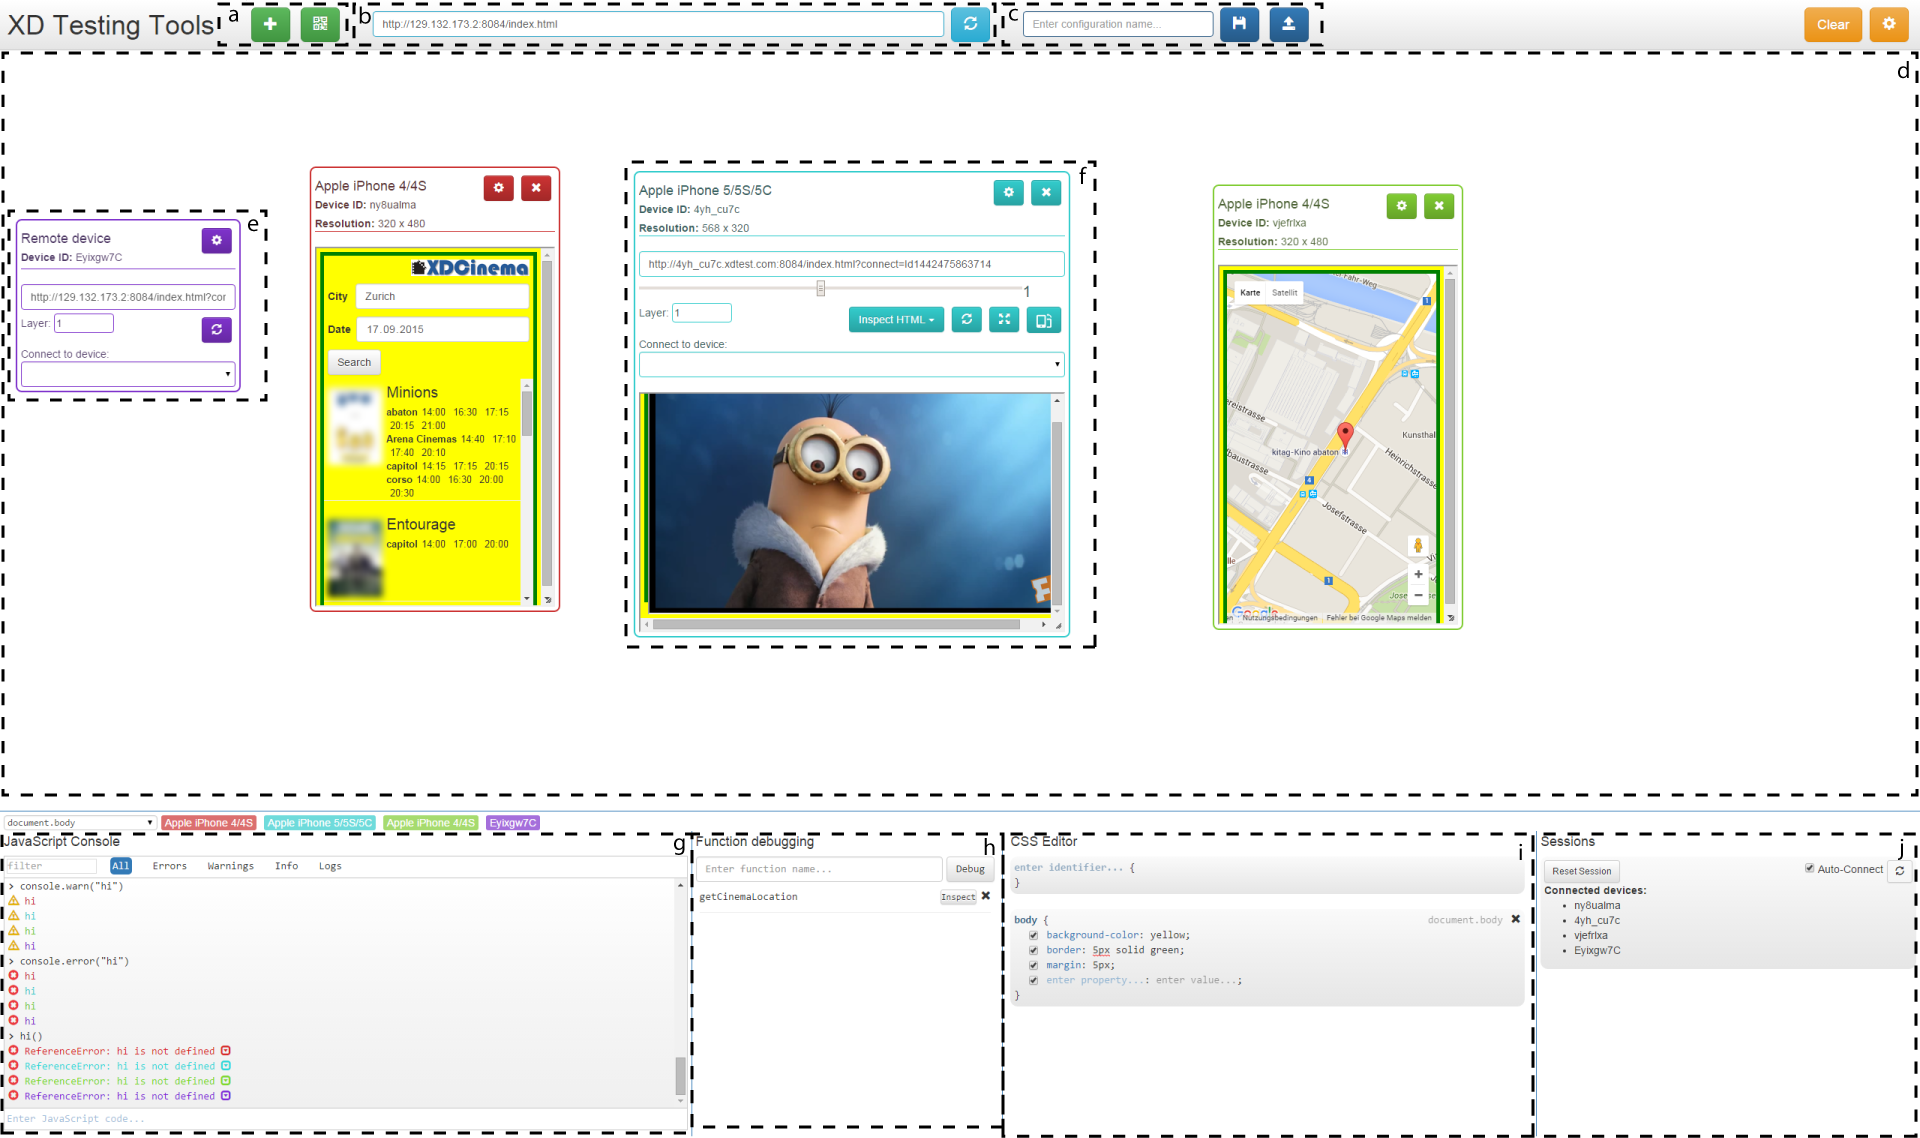
\includegraphics[width=1.0\textwidth]{images/screenshots/complete_labeled.png}
	\caption[Screenshot: Complete Interface]{The complete interface (without record and replay)}
	\label{fig:complete}
\end{figure}

The individual features of our system are labeled in the screenshot:
\begin{itemize}
	\item [a)] Buttons for adding emulated devices and showing the QR code for connecting real devices.
	\item [b)] Input field for loading a URL on all devices and button to refresh all devices.
	\item [c)] Loading and saving device configurations.
	\item [d)] Area where the devices can be positioned.
	\item [e)] Proxy of a connected real device.
	\item [f)] An emulated device.
	\item [g)] The shared JavaScript console.
	\item [h)] Function debugging.
	\item [i)] The shared CSS editor.
	\item [j)] Session management.
\end{itemize}

Figure~\ref{fig:complete_remote} shows a screenshot of the remote device that is connected to our system in the screenshot shown above.

\begin{figure}[H]
  \centering
    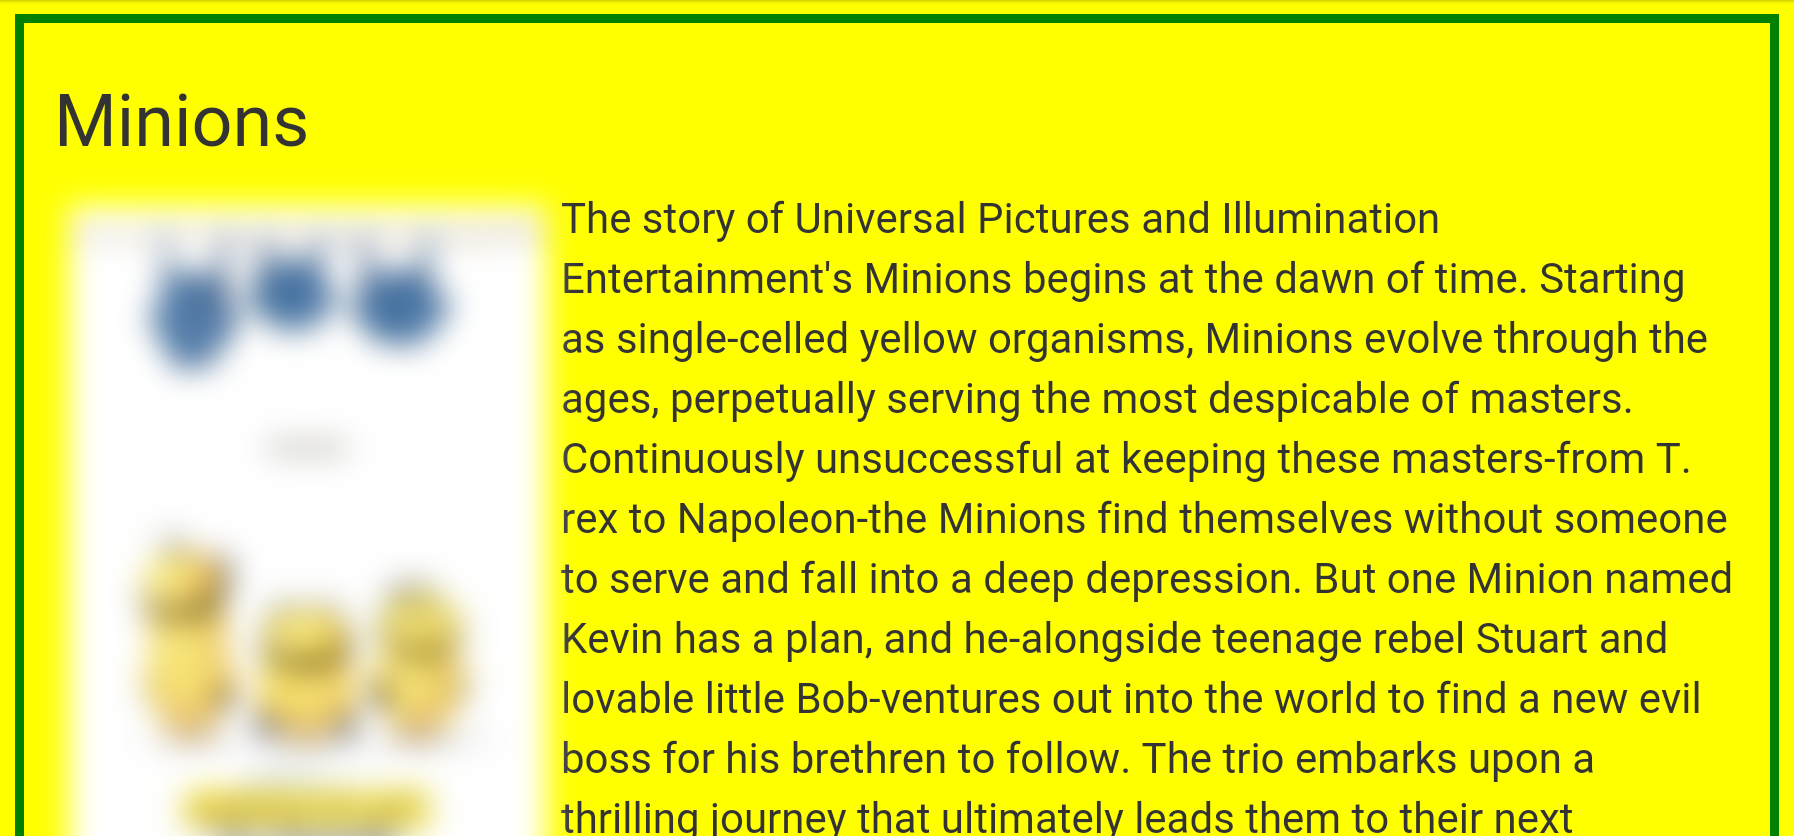
\includegraphics[width=0.8\textwidth]{images/screenshots/complete_remote_2.png}
	\caption[Screenshot: Remote Device]{The connected remote device}
	\label{fig:complete_remote}
\end{figure}

Our application also provides some options for disabling individual components The following components can be disabled:
\begin{itemize}
	\item Record and replay
	\item Shared JavaScript console
	\item Shared CSS editor
	\item Function debugging
	\item DNS server
\end{itemize}
The options are stored in the local storage of the browser. If a feature is disabled, the respective interface component is simply hidden. If the DNS server is disabled, the devices will just use the normal URL of the application. This will make it impossible to test the application with more than one emulated device, but if the developer prefers to use real devices anyway or does not have access to a local DNS server at the moment, disabling the server can be helpful. Furthermore, testing responsive web applications instead of cross-device applications would still be possible without the DNS server on emulated devices. The options also show all stored custom devices, device configurations and event sequences and allow the developer to delete any of them. A screenshot of the options can be seen in Figure~\ref{fig:options}.

\begin{figure}[H]
  \centering
    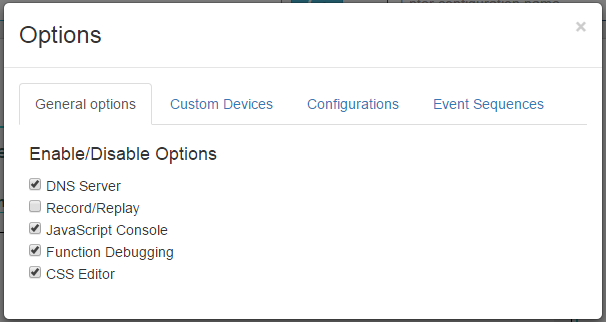
\includegraphics[width=0.9\textwidth]{images/screenshots/options.png}
	\caption[Screenshot: Options]{Options of our main application}
	\label{fig:options}
\end{figure}

Devices can also be activated and deactivated. If a device is inactive, it is not included in the following features:
\begin{itemize}
	\item Shared JavaScript console
	\item Shared CSS editor
	\item Function debugging
\end{itemize}
All those features perform some interactions with the devices automatically, thus they should be deactivated for inactive devices. Other features like record and replay still include inactive devices because manual interaction is needed anyway before something happens with the device. Devices can be activated and deactivated by clicking on their name/ID that is displayed above the JavaScript console, CSS editor and other stuff. When the device is active, the background of its name is in the color of the device, otherwise it is grey and the text color is in the color of the device. Figure~\ref{fig:active_inactive} illustrates the difference between active and inactive devices. The first device is inactive, the other two devices are active.

\begin{figure}[H]
  \centering
    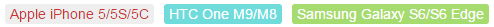
\includegraphics[width=0.8\textwidth]{images/screenshots/active_inactive.png}
	\caption[Screenshot: Active/inactive devices]{Active and inactive devices}
	\label{fig:active_inactive}
\end{figure}

\section{Emulation of Multiple Devices}

Devices are emulated with \lstinline|iframes|: Each emulated device is represented by its own \lstinline|iframe| that loads the application under test. However, loading the same domain inside multiple \lstinline|iframes| would lead to the sharing of session and persistent data between emulated devices. We have already described how developers tackle this problem and the limitations of those solutions. For our tools, we created a more scalable and robust solution. When an emulated device is created, it is assigned a unique ID. Based on this ID, a unique subdomain is registered with the local DNS server. All those subdomains point to the application under test, but as the application is accessed through different domains, no data is shared between the emulated devices. Domains that are unknown to the local DNS server are forwarded to the standard DNS server. The resolution of each \lstinline|iframe| corresponds to the resolution of the device that it represents in CSS pixels. Currently, only the resolution of the target devices is emulated, but in the future, our tools could be extended to support emulation of more aspects. In Figure~\ref{fig:emulated_device}, an emulated device can be seen.

\begin{figure}[H]
  \centering
    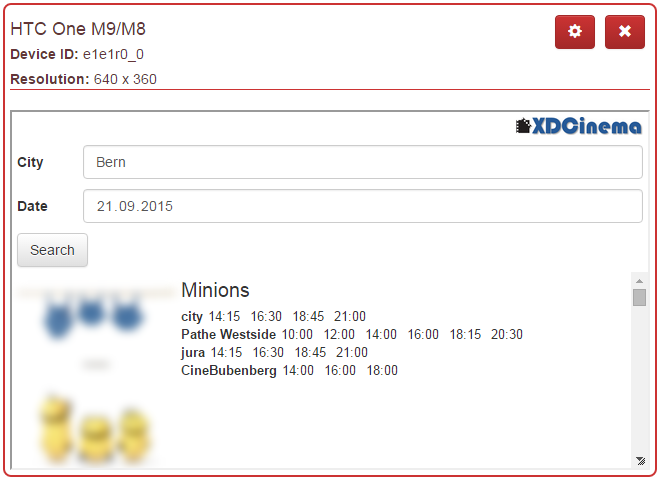
\includegraphics[width=0.8\textwidth]{images/screenshots/emulated_device_3.png}
	\caption[Screenshot: Emulated device]{An emulated device}
	\label{fig:emulated_device}
\end{figure}

Apart from its unique ID, each device also has a unique color. The border of the emulated device is colored with this color and the color is used in multiple other places for identifying the device. The devices also have a settings menu. In the settings menu, the developer can configure the following things:
\begin{itemize}
	\item The URL of the device.
	\item The scaling of the device.
	\item The orientation of the device.
	\item The layer of the device, i.e. the z-index. 
	\item The \lstinline|iframe| of the device can be refreshed.
	\item The developer can inspect the HTML of the device.
	\item The developer can connect the device to another device by choosing it from a dropdown menu.
\end{itemize}
The device's settings are not constantly used by the developer and showing them at all times would occupy valuable screen space. Thus, the setting menu can be extended and collapsed by clicking a button. The scaling of the device is set using the CSS property "transform", e.g. by setting "transform: scale(0.5)" to scale a device to half its usual size. Using the "transform" property does not change the resolution of the \lstinline|iframe| of the emulated device, only the space that the \lstinline|iframe| occupies. Thus, the layout of the emulated device remains intact even if it is scaled down. If the developer instead wants to change the resolution of a device, they can click in the bottom-right corner of the \lstinline|iframe| and drag to increase or decrease the resolution. An example of a settings menu can be seen in Figure~\ref{fig:settings_menu}. 

\begin{figure}[H]
  \centering
    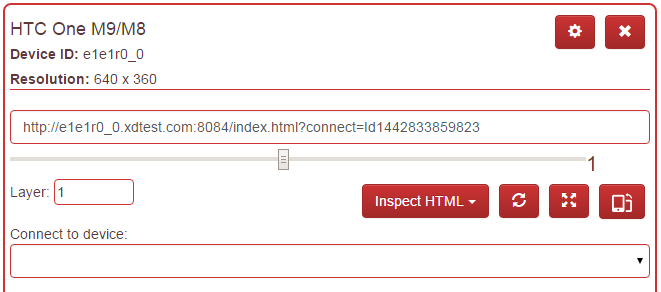
\includegraphics[width=0.8\textwidth]{images/screenshots/settings_menu_2.png}
	\caption[Screenshot: Settings menu emulated device]{Settings menu of an emulated device}
	\label{fig:settings_menu}
\end{figure}

In principle, the developer can add as many emulated devices as desired. The only limiting factor is the available screen space, but scaling can be used to solve this issue. 

The devices can be moved around as desired. Using HTML5's Drag and Drop, the developer can move the device by clicking on the header of the device and dragging it to the desired location. However, we cannot just make the devices \lstinline|draggable| by default. The developer should not be able to move the device if they click on the \lstinline|iframe| because otherwise interaction with the \lstinline|iframe| would be difficult. Thus, we chose to only make devices \lstinline|draggable| if the developer clicks on the header of the device. For this reason, we assign a click handler to each device that checks if the developer clicked on the header of the device. If they did, we make the device \lstinline|draggable|. 

When the developer starts dragging the device, the device ID is assigned as data to the event. However, the device ID is not the only required data. If the developer drags the device at a certain position, we cannot just assign this position to the device. If we did, the top left corner of the device would be at the position where the device was dropped, but the developer probably did not click on the top left corner of the device when they started dragging the device. Thus, we need to compute the offset of the click from the top left corner of the device and adjust the position accordingly when the device is dropped. For example, if the developer clicks on the device 10 pixels from the top and drops the device x pixels from the top of the device area, we need to assign the position x - 10 to the device. For achieving this, we compute the offset when the developer clicks on the header of a device and also set the offset as data to the event.

\subsection{Color Generation}
As described above, each device has its own unique color. We use the HSL\footnote{\url{https://en.wikipedia.org/wiki/HSL_and_HSV}} color space for determining device colors because finding distinct colors is a much simpler task in the HSL model compared to the RGB model. In the HSL color space, colors consist of three values: Hue, saturation and lightness. The colors of the devices should all have the same saturation and lightness, thus the only value that needs to be determined is the hue. The hue can have any value between 0 and 360. Our goal is to have colors that are easily distinguishable, thus their hues should be as different as possible. A simple algorithm can be used for determining the color of the next device:
\begin{itemize}
	\item If no colors have been assigned yet, assign the color 0/360.
	\item If only one color has been assigned, assign the color 180.
	\item If at least two colors have been assigned, compute the maximum distance between two assigned colors and assign the color in between.
\end{itemize}

\section{Easy Integration of Real Devices}

Real devices can be connected by scanning a QR code or opening a URL. When the URL is opened, the device loads the helper application. Once the helper application is loaded, the application under test is shown in a full-screen \lstinline|iframe| on the device. The developer can use the application on the real device, but everything relating to testing and debugging is coordinated through the main application. Therefore, no interface elements are required on the real device. Each connected real device is represented by a proxy within our main application. The proxy of the real device also contains a settings menu, but no \lstinline|iframe|. The settings menu is also missing a few things compared to emulated devices:
\begin{itemize}
	\item Scaling of the device: There is no need to scale real devices, as no \lstinline|iframe| is shown in the main application.
	\item Switching orientation: The orientation of a real device can be switched on the real device itself by simply rotating the real device.
	\item Inspecting the HTML: The main application has no access to the HTML of the real device, thus it cannot be inspected.
\end{itemize}
Figure~\ref{fig:settings_menu_remote} shows the settings menu of a remote device. The settings menu only contains interface elements for setting the URL of the device, refreshing the application under test, the layer input field and the dropdown menu for connecting the device to other devices. If the developer issues any command on the main device, e.g. refreshing the \lstinline|iframe| of the real device, the command is first sent to the server and then forwarded to the target device. 

\begin{figure}[H]
  \centering
    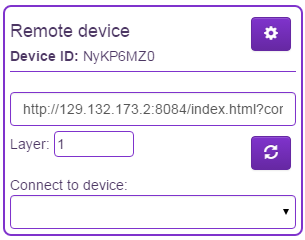
\includegraphics[width=0.5\textwidth]{images/screenshots/remote_device.png}
	\caption[Screenshot: Settings menu remote device]{Settings menu of a remote device}
	\label{fig:settings_menu_remote}
\end{figure}

The proxy of the real device can be moved around just like the emulated devices and its settings menu can also be collapsed and extended. Furthermore, each real device also has a unique ID and color for easy identification.

\section{Easy Switching of Device Configurations}

The developer can save different configurations of emulated devices. The developer can type the name of a device configuration into an input field and then either click a save button to save the current device configuration under that name or click a load button to load a device configuration with that name (if it exists). Autocomplete is used for providing suggestions for existing device configurations that could be loaded (see Figure~\ref{fig:session_management}). 

\begin{figure}[H]
  \centering
    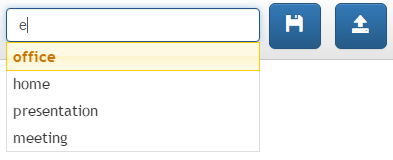
\includegraphics[width=0.6\textwidth]{images/screenshots/session_management_2.png}
	\caption[Screenshot: Saving/Loading device configurations]{Saving/Loading Device Configurations}
	\label{fig:session_management}
\end{figure}

Device configurations are stored in Local Storage. The Local Storage stores an array containing the names of all saved device configurations. This array is used for the autocomplete functionality and for retrieving the actual device configuration. The actual device configuration is an array of devices. For each device, the name, width, height, device pixel ratio, scaling, layer and position is stored. It does not make any sense to store real devices because they might not be available when the device configuration is loaded and they need to be re-connected manually anyway by opening the appropriate URL, thus only emulated devices are stored in device configurations. If the developer wants to load a device configuration, an ID is requested for each device, then the device is created and its scaling and position are set according to the values in the Local Storage.

\section{Integration with Debugging Tools}

Our system includes a few different features that are also available in normal browser debugging tools. Those features work in a similar way as in the browser, but we extended them to support debugging of multiple devices at the same time.

\subsection{Shared JavaScript Console}

The shared JavaScript console aggregates the console output (logging and JavaScript errors) of all devices and allows the developer to send commands to all devices. The following types of logging messages are aggregated:
\begin{itemize}
	\item \lstinline|console.log|
	\item \lstinline|console.debug|
	\item \lstinline|console.warn|
	\item \lstinline|console.info|
	\item \lstinline|console.error|
	\item \lstinline|console.count|
	\item \lstinline|console.dir|
	\item \lstinline|console.assert|
\end{itemize}
In the script that is injected in the application under test, those functions are overwritten by a new function and the original functions are stored. The new function performs the following two actions: First, it sends the content and type of the logging message to our server. Second, it calls the original logging function. Thus, the logging messages are still displayed in the standard console, but are forwarded to our console in addition.

Apart from forwarding logging messages, we also forward JavaScript errors. This is implemented by assigning an event handler to JavaScript errors using \lstinline|window.onerror|. Whenever a JavaScript error occurs, the event handler is called. Inside the event handler, the JavaScript error message is sent to our server, together with the stack trace if available. 

All messages are assigned to one of four categories:
\begin{itemize}
	\item Warnings: This includes all logging messages that use "console.warn".
	\item Errors: This includes all logging messages that use "console.error", JavaScript errors and assertion failures in "console.assert".
	\item Info: This includes all logging messages that use "console.info".
	\item Log: This includes all other types of messages.
\end{itemize}
Depending on the type of message, a different symbol is used in front of the message when it is displayed in the shared JavaScript console. The message itself is colored in the color of the device that sent it. If a device is deactivated, it does not forward any messages or errors anymore and all existing messages are filtered out until the device is activated again. 

The messages in the console can also be filtered: The developer can either filter the messages by type of message, e.g. show only all error messages, or by text. If the console messages are filtered by text, all messages that do not contain the text to filter by anywhere are hidden. If the filter is removed, the hidden messages are shown again.

When a JavaScript error with stack trace is received by the console, the stack trace is split into multiple lines where each line represents one entry of the stack trace. By default, the developer only sees the error message itself without the stack trace. By clicking on a down-arrow button next to the error message, the developer can extend and collapse the stack trace. Figure~\ref{fig:stack_trace} shows what such a stack trace looks like in our JavaScript console.

\begin{figure}[H]
  \centering
    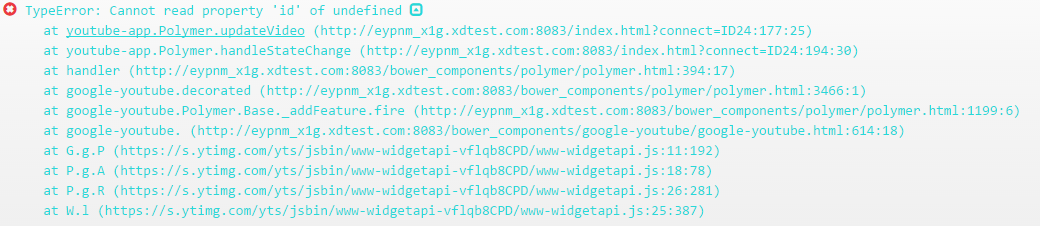
\includegraphics[width=1.0\textwidth]{images/screenshots/stack_trace.png}
	\caption[Screenshot: Stack trace]{Stack trace}
	\label{fig:stack_trace}
\end{figure}

If the developer wants to send a command to the devices, they can type the command into an input field below the console and press the enter key. The command is then sent to all active devices. When the command is received by the device, the device calls \lstinline|eval| with the command string as argument. The return value of the command is sent back to the main application and displayed in the console.

The shared JavaScript console also has a history function similar to the console in Chrome DevTools. Whenever the user types a command, the command is stored in an array containing the command history. By using the arrow keys, the developer can navigate through this array and call previous commands again.

The screenshot in Figure~\ref{fig:js_console} shows the shared JavaScript console including a few examples of how to use it. First, the developer tries to call a function on all devices but makes a typo. Because the function with the typo in the name does not exist, an error message is displayed by all devices. The developer then notices the typo, types the correct function and sees the return values of the function (the coordinates of a cinema). Finally, the developer wants to see which roles have been assigned to the devices. They type the name of the variable that contains the roles and the value of this variable on all devices is shown in the console.

\begin{figure}[H]
  \centering
    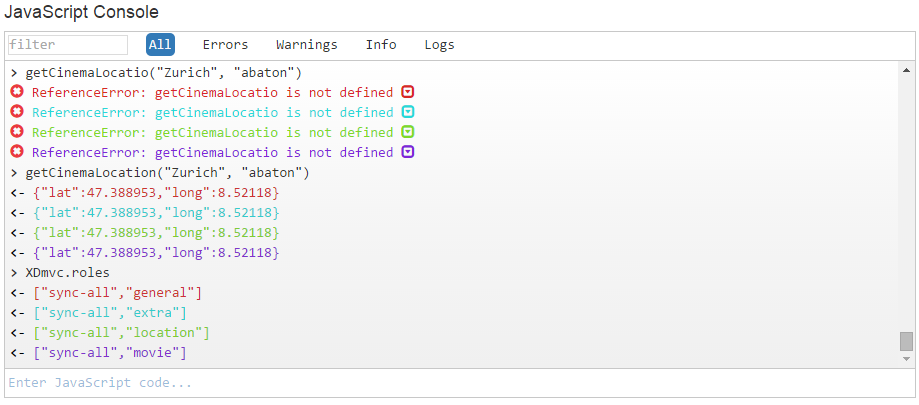
\includegraphics[width=1.0\textwidth]{images/screenshots/js_console_2.png}
	\caption[Screenshot: JavaScript console]{Shared JavaScript console}
	\label{fig:js_console}
\end{figure}

\subsection{Function Debugging and Inspection}

Function debugging and inspection requires the Chrome extension. When the developer opens the Chrome DevTools, a new area is displayed at the bottom of our main application. In this area, the developer has access to an input field where they can type the name of the function they want to debug.  Below the input field, the list of functions that are currently debugged is shown. When the developer adds a new function to debug, a command is sent to each activated emulated device. If a device receives the name of a function to debug, it overwrites the function to debug by a new function and stores the original function. The function that overwrites the original function performs the following actions:
\begin{enumerate}
	\item It highlights the device with a semi-transparent green overlay.
	\item It calls the original function and stores the return value.
	\item It removes the highlighting from the device.
	\item It returns the return value.
\end{enumerate}
After overwriting the original function, the device sends a message back to the main application that it is ready for debugging. The main application then sends a command to the Chrome extension with the name of the variable that stores the original function. The Chrome extension receives the command and the URL of the device the message originated from. The Chrome extension then calls the "debug" function with the function name and the URL of the frame that represents the device. Debugging a function is roughly equivalent to setting a breakpoint at the beginning of the function: Whenever the function is called, the debugger pauses at the beginning of the function and the developer can perform their debugging actions.

When a debugged function is called on any of the active devices, the overwriting function is called first and highlights the device. Then, the original function is called and interrupted right at the beginning so the developer can debug the function. After finishing debugging, the function call returns and the device is unhighlighted. Figure~\ref{fig:function_debugging_complete} shows a screenshot while a function is being debugged. In the screenshot, the highlighted device, the DevTools with the debugged function open and the list of debugged functions can be seen.

\begin{figure}[H]
  \centering
    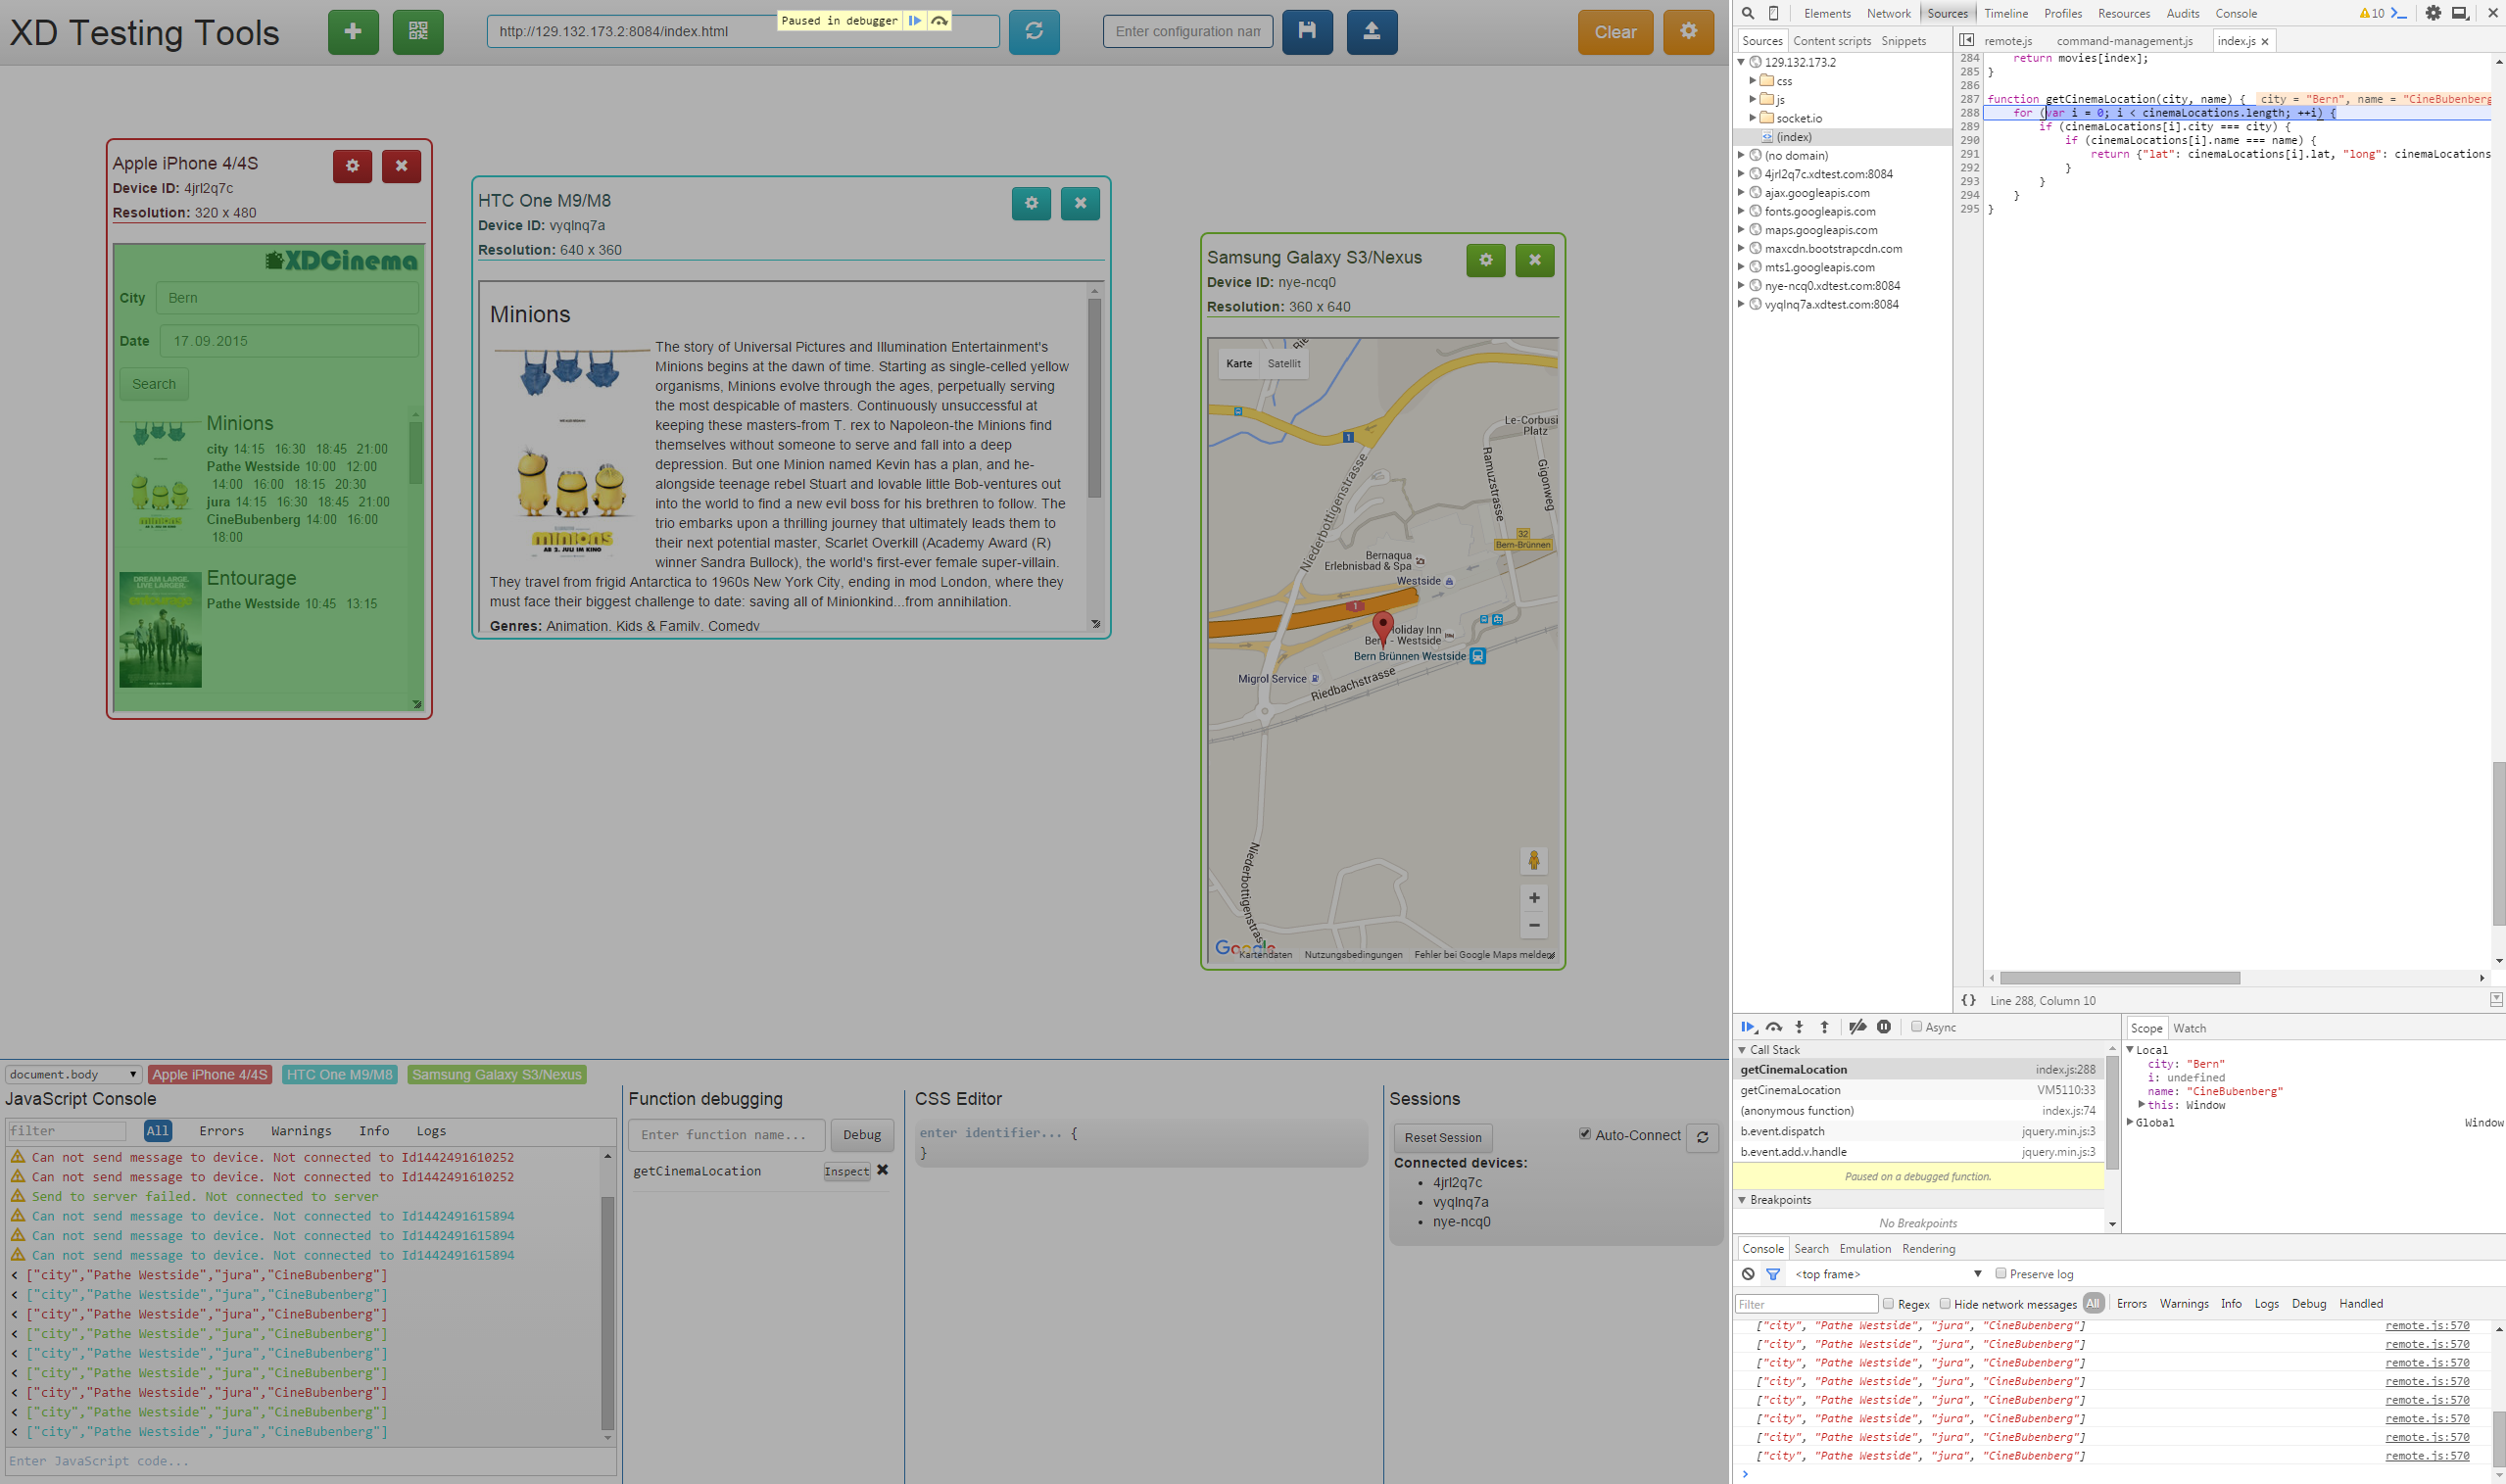
\includegraphics[width=1.0\textwidth]{images/screenshots/function_debugging_complete.png}
	\caption[Screenshot: Function debugging]{The complete interface while debugging a function}
	\label{fig:function_debugging_complete}
\end{figure}

If the developer is done debugging a function, they can remove it from the list of debugged functions and the original function is restored inside the script. Then, a command is sent to the DevTools extension, informing it to stop debugging the function. 

The developer can also just inspect the function without it being called by clicking on a button next to the function name in the list of debugged functions. If this button is called, an emulated device is picked at random and the function is opened on this device by sending a command to the DevTools extension. 

The functions that are debugged run inside an \lstinline|iframe| and the URL of the \lstinline|iframe| needs to be passed as a parameter. However, when a new device is added, the hook for the \lstinline|iframe| of the new device does not exist yet and the Chrome DevTools need to be closed and re-opened. Similarly, if the URL of a device changes, the hook is lost. Unfortunately, there is no way of automatically re-opening the DevTools. For this reason, a red overlay containing a warning text is shown whenever a URL changes or a new device is added. The warning can be seen in Figure~\ref{fig:warning}.

\begin{figure}[H]
  \centering
    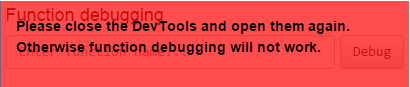
\includegraphics[width=0.7\textwidth]{images/screenshots/warning.png}
	\caption[Screenshot: Function debugging warning]{Warning that is shown for function debugging}
	\label{fig:warning}
\end{figure}

\subsection{HTML Inspection}

HTML inspection also requires the Chrome extension and thus only works on emulated devices. Inside the settings menu of each emulated device, a button can be clicked to inspect the HTML of the device. If the button is clicked, a command is sent to the DevTools extension, telling it to open the \lstinline|body| element of the frame with the URL of the device. The HTML inspection view in the Chrome DevTools then jumps directly to the body of the HTML of the device.

\subsection{Shared CSS Editor}

The shared CSS editor adds CSS rule to all active devices. Inside the injected script of the application under test, a stylesheet is created and added to the DOM tree. When the developer adds a new rule to the CSS editor, a command is sent to all active devices and the rule is added to an array containing all CSS rules. Whenever the array with the CSS rules changes, the stylesheet is rewritten. Retrieving the appropriate rule from the stylesheet and modifying it is difficult and time-consuming, simply rewriting the stylesheet is much more convenient, especially since we do not expect developers to add hundreds of rules to the shared CSS editor. The developer can also disable rules and enable them again later. If a rule is disabled, it is removed from the stylesheet; if it is enabled again, it is re-added to the stylesheet. The developer can also modify the CSS rules in the shared CSS editor. 

The CSS editor also has some autocomplete functionality: If the developer starts typing the name of a property, the property is automatically completed using the first CSS property name that matches the text typed by the developer (see Figure~\ref{fig:css_autocomplete}.

\begin{figure}[H]
  \centering
    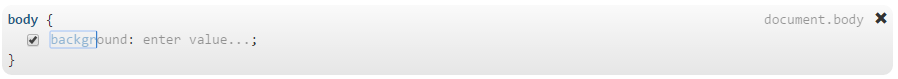
\includegraphics[width=1.0\textwidth]{images/screenshots/css_autocomplete.png}
	\caption[Screenshot: CSS editor autocomplete]{Autocomplete in the CSS editor}
	\label{fig:css_autocomplete}
\end{figure}
The available CSS properties are retrieved using "document.body.style" which contains all available CSS properties, even if they are not set. The CSS properties of \lstinline|document.body.style| are then converted to an array of available CSS properties.

Figure~\ref{fig:css_editor} shows a screenshot of the CSS editor in action. In this screenshot, some CSS rules are added to the \lstinline|body| element of all devices.

\begin{figure}[H]
  \centering
    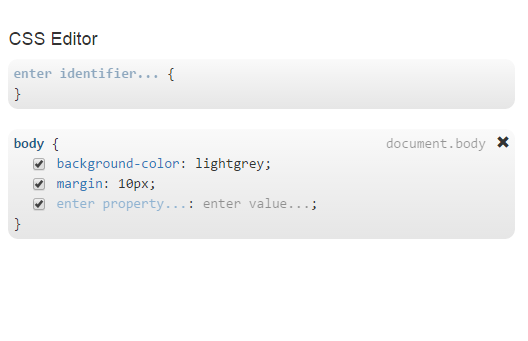
\includegraphics[width=1.0\textwidth]{images/screenshots/css_editor.png}
	\caption[Screenshot: CSS editor]{Shared CSS Editor}
	\label{fig:css_editor}
\end{figure}

In Figure~\ref{fig:css_applied}, the effects of the CSS shown in the screenshot above are shown. 

\begin{figure}[H]
  \centering
    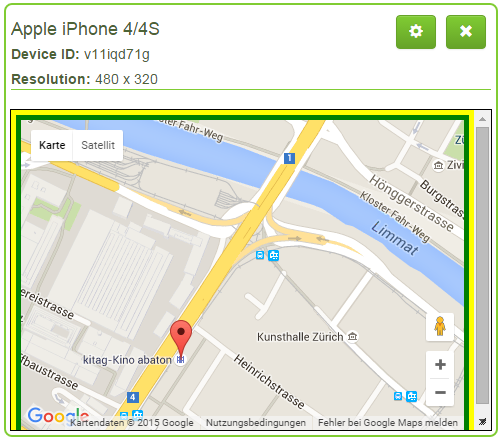
\includegraphics[width=0.5\textwidth]{images/screenshots/emulated_device_4.png}
	\caption[Screenshot: CSS effects]{CSS applied to emulated device}
	\label{fig:css_applied}
\end{figure}

\section{Automatic Connection Management}

The devices in our system can either be connected automatically or manually. Each set of connected devices represents a session. For each session, a checkbox allows the developer to toggle on or off auto-connect. When the first device is created or connected, auto-connect is turned on by default. If auto-connect is on, all newly created and connected devices will automatically be connected to that session. Thus, if the developer simply adds or connects a number of devices, they will automatically all be connected. If the developer wants to have multiple sessions, they can turn off auto-connect and then add more devices. Each device also has a drop-down menu in its settings menu for manually connecting to other devices. 

All current sessions are displayed at the bottom of the page of our application. Each session displays all connected devices (see Figure~\ref{fig:sessions}). The developer can also refresh all devices in a session and reset a session. Resetting a session assigns new IDs to all devices and thus erases the data of the devices. 

\begin{figure}[H]
  \centering
    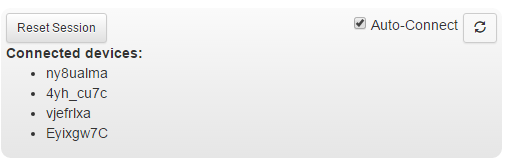
\includegraphics[width=0.6\textwidth]{images/screenshots/session_management.png}
	\caption[Screenshot: Session]{A device session}
	\label{fig:sessions}
\end{figure}

In the script that is injected into the testing application, a connection function is available. When a device wants to connect to another device, a command is sent to that device. That device then calls the connection function. The connection function returns the URL that has to be loaded to connect to the device. The URL is then sent back to the device that wants to connect and can be loaded to connect the device.

The URL required for connecting depends on the application. Thus, the developer has to adjust the connection function such that it returns the appropriate URL. So far, only connecting via URL is supported, but extending the connection function to support other connection mechanisms would be possible.

\section{Coordinated Record and Replay}

Record and replay records all user interactions with the application under test and allows the developer to replay them. Recording is done by assigning event handlers for all relevant events that we want to record. It is important that no-one receives the recorded events before us, because otherwise they could modify the page or even stop event propagation. For this reason, the event handlers are assigned as soon as the injected script is loaded. However, the event handlers do not do anything as long as recording has not started yet. When the developer starts recording, all events are logged to an array. After finishing recording, the array of events is sent to the main application. 

Furthermore, all event handlers are capturing and are assigned to the document itself. Since no other element in the DOM hierarchy can be above the document element, the document element is always the first element that receives an event with capturing event handlers. After finishing recording and before sending the event sequence back to the server, all circular structures are removed. All other event properties are kept so the events can be replayed accurately.

The event sequences should be replayable on other devices than the recording devices, therefore some way of determining the target of the event is required. Whenever an event handler is triggered, the DOM hierarchy is traveled up from the target of the event until an ID is reached. From this ID, we can determine the target element by taking the correct child until the target element is reached. From this, we can derive a hierarchy that describes how to reach the target element on a device and replaying the event on another device becomes possible.

After the main application receives an event sequence, the sequence is visualized. Drag and drop can be used to adjust the timing of the event sequences on the devices. Event sequences can also be moved to other devices using drag and drop. Event sequences can be saved to local storage for later use. Because all events require some space when visualized, events that happen close together in time are grouped together. Event sequences can also be split by clicking between two groupings of events. Figure~\ref{fig:record_replay} shows how event sequences are visualized.

\begin{figure}[H]
  \centering
    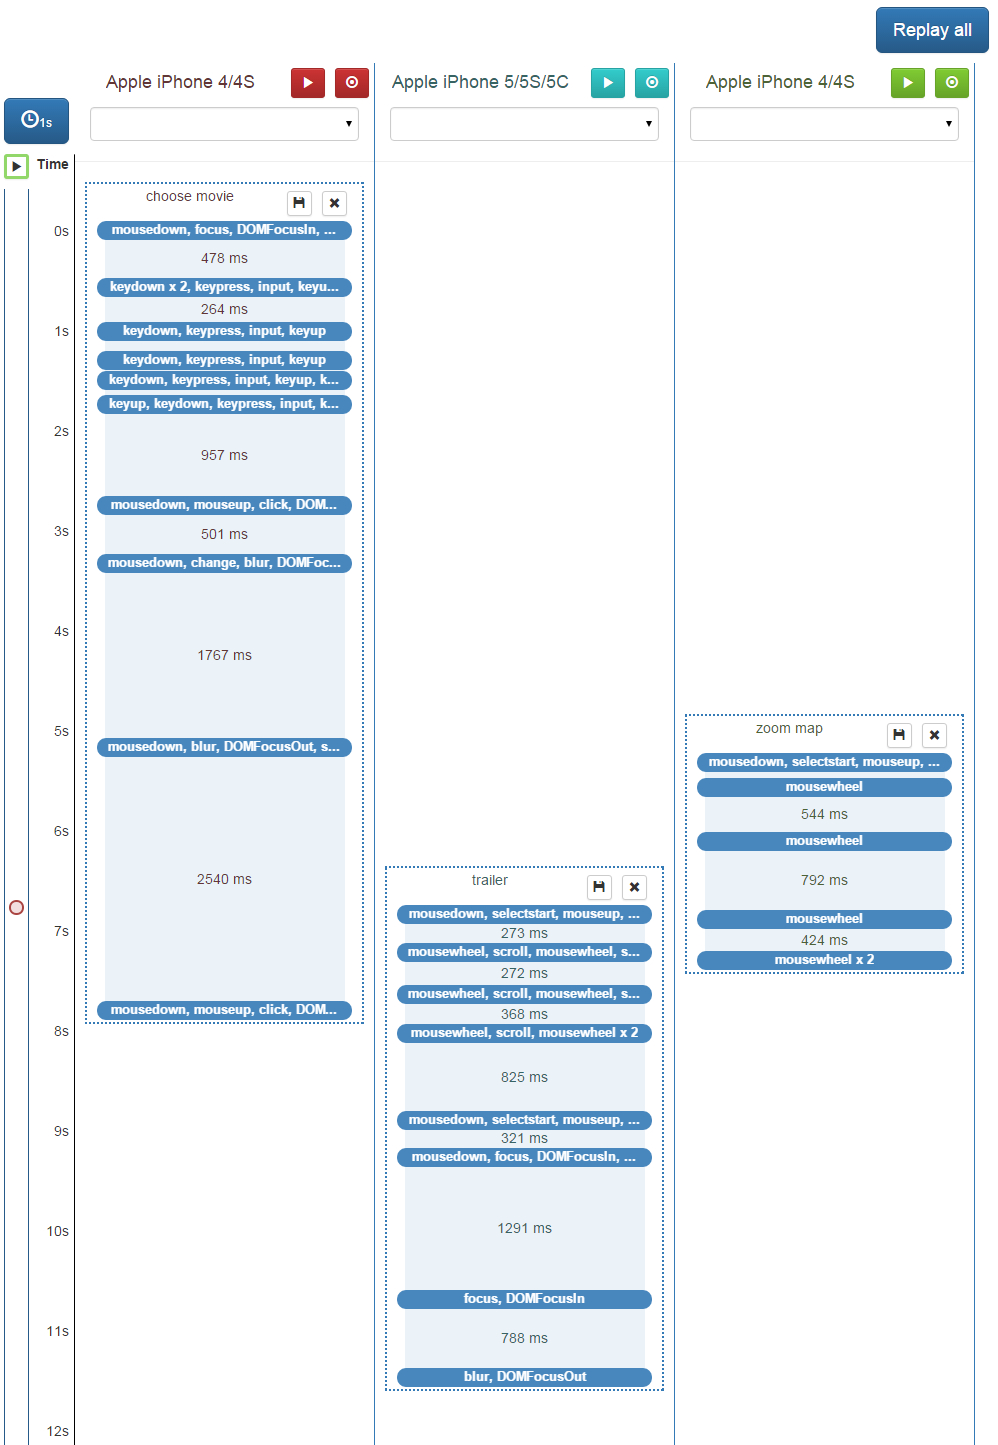
\includegraphics[width=1.0\textwidth]{images/screenshots/record_replay.png}
	\caption[Screenshot: Record and replay]{Record and Replay}
	\label{fig:record_replay}
\end{figure}

Furthermore, the developer can add breakpoints to the timing of the replay. Next to the event visualizations, a timeline is shown as well as a narrow empty column where the developer can click to add a breakpoint at a certain point in time. When the developer starts replaying, the event sequences assigned to a device are sent to the device along with the list of breakpoints. The events that happen before the first breakpoint are then triggered using \lstinline|setTimeout|. If a breakpoint is reached, a message is sent to the main application and the breakpoint that was reached is highlighted. After the developer chooses to continue, a message is sent to all replaying devices telling them to continue event replaying until the next breakpoint is reached. After the last breakpoint has been reached, the event replaying continues until all events have been replayed. The developer can either choose to replay only on one specific device or on all devices simultaneously. 

All events are replayed using the properties recorded in the event sequences. Using the hierarchy computed when recording, the target element of the event is determined. For most events, replaying with the properties logged when recording is enough for realistically reproducing the events. However, some events require a bit more work. Replaying key events is possible, but no text is written into input fields. In addition to the key events, we also need to trigger a text event using the correct char code. Scrolling events also do not scroll. Thus, we also log the scrolling position after a scrolling event occurs and manually set it after replaying the event. Furthermore, the backspace key cannot be reproduced with neither text events nor key events. Thus, we manually determine the position of the caret if the backspace key is pressed and delete the last character before the caret when replaying. 

\section{Integration with Polymer and Shadow DOM}

Although our system works with all web-based cross-device applications, one of the initial goals was to make it work with applications developed with XD-MVC. XD-MVC can either just be used as a JavaScript API or it can be used together with Polymer\footnote{\url{https://www.polymer-project.org}}. Polymer provides developers with the option to use Shadow DOM\footnote{\url{http://www.w3.org/TR/shadow-dom/}}. Shadow DOM refers to the ability of the browser to include a subtree of DOM elements into the rendering of the document, but not into the main document tree. Thus, it can encapsulate components and prevent them from being reached by traditional tree walking functions such as \lstinline|childNodes| and \lstinline|firstChild|. We must assume that some applications implemented with XD-MVC use Polymer and Shadow DOM and our system should support those applications as well. However, a few modifications are required for supporting both Polymer and Shadow DOM. First, determining the target of an event can become more difficult because the element might not be accessible from the global scope. Second, debugging functions that are not accessible from the global scope should be possible and we need some way of accessing those functions. Furthermore, we want to be able to add CSS to elements that are not accessible from the global scope.

\subsection{Determining Event Targets}

An element can define Shadow DOM by attaching a shadow root to itself. The shadow DOM can be accessed using the \lstinline|shadowRoot| property of the element. Without Shadow DOM, finding the nearest element with an ID was enough for determining the path that leads to the target element of an event. With Shadow DOM, we need to additionally consider all shadow roots that lead from the \lstinline|body| element to the target element. The \lstinline|path| property of the event contains all elements that were visited by the event. We adjusted our algorithm in the following way:
\begin{enumerate}
	\item Take the lowest (in the DOM hierarchy) element in the path that has not yet been processed.
	\item Determine how to reach this element from the next higher element in the path:
	\begin{enumerate}
		\item Check if the element has a parent node. If not, it must be the hierarchically highest element inside a shadow root. Thus, it can be reached by accessing the \lstinline|shadowRoot| property of the higher element.
		\item Check if the element has an ID. If yes, it can be reached using the ID.
		\item If the element has a parent element but no ID, it can be accessed by accessing the appropriate child of the parent element.
	\end{enumerate}
	\item Go back to Step 1.
\end{enumerate}
Using this hierarchy, the target element can already be reached, but because of elements with ID, some steps can be skipped. Inside each shadow root, we look for the lowest element with an ID. All elements inside the shadow root but above that element can be skipped and the ID can be accessed directly. If no element has an ID, we have to keep all elements. The same can be done for the path from the \lstinline|body| element to the highest shadow root and for the path from the lowest shadow root to the target element. Using this algorithm, the shortest path to the target element is computed. For applications that do not contain any Shadow DOM, the algorithm yields the same result as the standard algorithm described earlier. The computed hierarchy can be used to determine the target of the event on other devices by accessing shadow roots instead of IDs or children when appropriate.

This modified algorithm allows us to record and replay events on applications that use Shadow DOM. 

\subsection{Determining Scopes}

There are two things to be considered: First, there may be shadow roots in the application. Second, the developer can define functions for their custom Polymer elements that need to be accessed using the Polymer element. In principle, those functions can be accessed using the appropriate path through the DOM tree, but determining this path is not trivial. Thus, we want to automatically determine all different scopes on which functions can be defined, i.e. all shadow roots and Polymer elements and the path through the DOM tree that leads to those scopes. We implemented the following algorithm for determining the scopes:
\begin{enumerate}
	\item Add the \lstinline|body| element to the processing queue.
	\item As long as the processing queue is not empty, take the first element and perform the following actions:
		\item If the element has the property \lstinline|shadowRoot|, we found a new scope and add it to the list of scopes, together with the path that determines how to reach the scope. Then we add the shadow root of the element to the processing queue.
		\item If the element has the property \lstinline|is|, it is a Polymer element and we add it to the list of scopes, together with the path. Then we add each child of the element to the processing queue.
		\item If neither of the above is true, we have not found a new scope and we simply add all children of the element to the processing queue.
\end{enumerate}
When the algorithm has finished, the list of scopes is sent to the main application. In the main application, the developer can choose the scope that they want to work with from a dropdown menu.

The selected scope has an influence on the following three components of our system:
\begin{itemize}
	\item Shared JavaScript console: In the shared JavaScript console, all commands in the console are executed in the selected scope. 
	\item Shared CSS editor: In the CSS editor, the CSS rule is added on the currently selected scope. Each scope has its own stylesheet containing the CSS rules of that scope.
	\item Function debugging: The functions that are debugged are on the selected scope.
\end{itemize}